\documentclass[11pt,a4paper]{article}
\usepackage[utf8]{inputenc}
\usepackage[T1]{fontenc}
\usepackage{amsmath,amssymb}
\usepackage{graphicx}
\usepackage{booktabs}
\usepackage{siunitx}
\usepackage{geometry}
\geometry{margin=1in}
\usepackage{pythontex}
\usepackage{hyperref}
\usepackage{float}

\title{Signal Detection\\d-prime and ROC}
\author{Psychophysics Research Group}
\date{\today}

\begin{document}
\maketitle

\begin{abstract}
Signal Detection Theory (SDT) provides a mathematical framework for quantifying perceptual sensitivity and decision criteria in psychophysical tasks. This report implements computational methods to calculate detectability ($d'$), response bias ($\beta$ and $c$), and receiver operating characteristic (ROC) curves. Using Gaussian signal and noise distributions, we analyze hit rates, false alarm rates, and criterion placement under varying task conditions. Applications include sensory perception, medical diagnosis, and quality control decision-making.
\end{abstract}

\section{Introduction}

Signal Detection Theory (SDT) separates an observer's sensitivity to detect a signal from their response bias when making binary decisions under uncertainty \cite{Green1966,Macmillan2005}. Unlike classical psychophysics, which assumes a fixed threshold, SDT recognizes that both signal strength and decision strategy influence detection performance \cite{Swets1961}.

The theory assumes two overlapping Gaussian distributions: noise alone ($N$) and signal-plus-noise ($S+N$). The separation between these distributions defines sensitivity ($d'$), while the decision criterion ($\lambda$) determines response bias. This framework applies broadly to perception \cite{Wickens2002}, memory \cite{Yonelinas2002}, and medical diagnosis \cite{Metz1978}.

We implement computational methods to:
\begin{itemize}
    \item Calculate $d'$ from hit and false alarm rates
    \item Visualize signal and noise distributions
    \item Generate ROC curves for multiple sensitivity levels
    \item Compute likelihood ratio ($\beta$) and criterion ($c$)
    \item Analyze z-transform relationships
\end{itemize}

\begin{pycode}

import numpy as np
import matplotlib.pyplot as plt
from scipy.stats import norm
from scipy import optimize, integrate
plt.rcParams['text.usetex'] = True
plt.rcParams['font.family'] = 'serif'

\end{pycode}

\section{Mathematical Framework}

The noise distribution is $N \sim \mathcal{N}(0, \sigma^2)$, and the signal-plus-noise distribution is $S+N \sim \mathcal{N}(\mu_s, \sigma^2)$. Sensitivity is quantified by:

\begin{equation}
d' = \frac{\mu_s - \mu_n}{\sigma} = \frac{\mu_s}{\sigma}
\end{equation}

Given an observer's hit rate $H = P(\text{``yes''} | \text{signal})$ and false alarm rate $F = P(\text{``yes''} | \text{noise})$, we estimate $d'$ using:

\begin{equation}
d' = z(H) - z(F)
\end{equation}

where $z(\cdot)$ is the inverse cumulative normal distribution (z-transform).

The decision criterion $\lambda$ defines the threshold for responding ``yes.'' The likelihood ratio at the criterion is:

\begin{equation}
\beta = \frac{f_{S+N}(\lambda)}{f_N(\lambda)} = \frac{\phi(\lambda - d')}{\phi(\lambda)}
\end{equation}

A bias-free criterion ($c = 0$) maximizes accuracy when signal and noise are equally likely.

\begin{pycode}
# Signal and noise distributions
x = np.linspace(-4, 6, 300)
d_prime = 2.0  # Sensitivity parameter
mu_noise = 0.0
mu_signal = d_prime
sigma = 1.0

noise_dist = norm.pdf(x, loc=mu_noise, scale=sigma)
signal_dist = norm.pdf(x, loc=mu_signal, scale=sigma)

# Decision criterion
criterion = 1.0  # Midpoint between means
criterion_height = max(norm.pdf(criterion, loc=mu_noise, scale=sigma),
                       norm.pdf(criterion, loc=mu_signal, scale=sigma))

# Calculate hit and false alarm rates for this criterion
hit_rate = 1 - norm.cdf(criterion, loc=mu_signal, scale=sigma)
false_alarm = 1 - norm.cdf(criterion, loc=mu_noise, scale=sigma)

# Likelihood ratio (beta)
beta = norm.pdf(criterion, loc=mu_signal, scale=sigma) / norm.pdf(criterion, loc=mu_noise, scale=sigma)

# Bias parameter c
c = -0.5 * (norm.ppf(hit_rate) + norm.ppf(false_alarm))

fig, ax = plt.subplots(figsize=(10, 6))
ax.plot(x, noise_dist, 'b-', linewidth=2.5, label='Noise ($N$)')
ax.plot(x, signal_dist, 'r-', linewidth=2.5, label='Signal + Noise ($S+N$)')
ax.fill_between(x, 0, noise_dist, where=(x >= criterion), color='blue', alpha=0.2, label=f'False Alarm = {false_alarm:.3f}')
ax.fill_between(x, 0, signal_dist, where=(x >= criterion), color='red', alpha=0.2, label=f'Hit Rate = {hit_rate:.3f}')
ax.axvline(criterion, color='black', linestyle='--', linewidth=2, label=f'Criterion $\\lambda$ = {criterion}')
ax.set_xlabel('Evidence Strength', fontsize=12)
ax.set_ylabel('Probability Density', fontsize=12)
ax.set_title(f"Signal and Noise Distributions ($d'$ = {d_prime}, $\\beta$ = {beta:.2f}, $c$ = {c:.2f})", fontsize=13)
ax.legend(loc='upper right', fontsize=10)
ax.grid(True, alpha=0.3)
ax.set_xlim(-4, 6)
plt.tight_layout()
plt.savefig('signal_detection_plot1.pdf', dpi=150, bbox_inches='tight')
plt.close()
\end{pycode}

\begin{figure}[H]
\centering
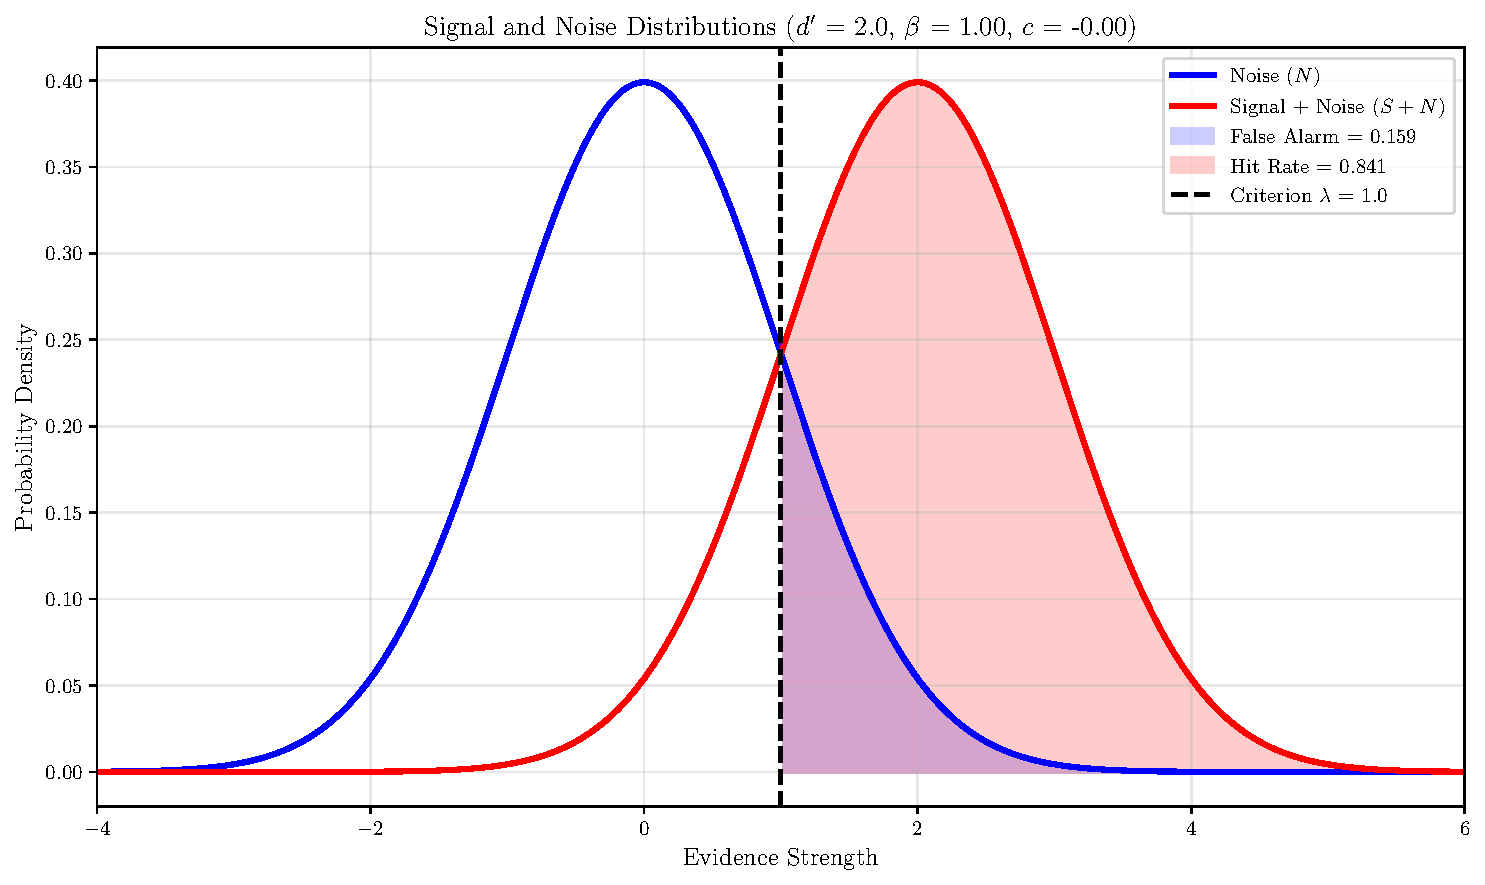
\includegraphics[width=0.95\textwidth]{signal_detection_plot1.pdf}
\caption{Gaussian signal and noise distributions with decision criterion at $\lambda = \py{criterion}$. The noise distribution (blue) is centered at $\mu_N = 0$, while the signal-plus-noise distribution (red) is centered at $\mu_S = \py{d_prime}$. The criterion divides the evidence axis into ``no'' (left) and ``yes'' (right) response regions. Shaded areas represent false alarm probability (blue) and hit rate (red). Sensitivity $d' = \py{d_prime}$ quantifies distribution separation, while likelihood ratio $\beta = \py{round(beta, 2)}$ and bias $c = \py{round(c, 2)}$ characterize the observer's decision strategy.}
\end{figure}

\section{Hit Rate and False Alarm Rate Analysis}

As the decision criterion $\lambda$ varies, hit rate $H(\lambda)$ and false alarm rate $F(\lambda)$ change in opposite directions. A liberal criterion (low $\lambda$) increases both $H$ and $F$, while a conservative criterion (high $\lambda$) decreases both.

For a fixed $d'$:
\begin{equation}
H(\lambda) = 1 - \Phi\left(\frac{\lambda - d'}{\sigma}\right), \quad F(\lambda) = 1 - \Phi\left(\frac{\lambda}{\sigma}\right)
\end{equation}

where $\Phi(\cdot)$ is the cumulative distribution function of the standard normal.

\begin{pycode}
# Vary decision criterion
criteria = np.linspace(-2, 4, 100)
d_prime_fixed = 2.0

hit_rates = 1 - norm.cdf(criteria, loc=d_prime_fixed, scale=1)
false_alarm_rates = 1 - norm.cdf(criteria, loc=0, scale=1)

# Calculate beta and c for each criterion
betas = norm.pdf(criteria, loc=d_prime_fixed, scale=1) / norm.pdf(criteria, loc=0, scale=1)
c_values = -0.5 * (norm.ppf(np.clip(hit_rates, 0.001, 0.999)) + norm.ppf(np.clip(false_alarm_rates, 0.001, 0.999)))

fig, (ax1, ax2) = plt.subplots(1, 2, figsize=(12, 5))

# Left: Hit rate and false alarm rate vs criterion
ax1.plot(criteria, hit_rates, 'r-', linewidth=2.5, label='Hit Rate $H(\\lambda)$')
ax1.plot(criteria, false_alarm_rates, 'b-', linewidth=2.5, label='False Alarm Rate $F(\\lambda)$')
ax1.axvline(d_prime_fixed/2, color='black', linestyle='--', linewidth=1.5, alpha=0.5, label='Optimal $\\lambda$ (unbiased)')
ax1.set_xlabel('Decision Criterion $\\lambda$', fontsize=12)
ax1.set_ylabel('Probability', fontsize=12)
ax1.set_title(f'Hit and False Alarm Rates vs. Criterion ($d\'$ = {d_prime_fixed})', fontsize=12)
ax1.legend(fontsize=10)
ax1.grid(True, alpha=0.3)
ax1.set_xlim(-2, 4)
ax1.set_ylim(0, 1)

# Right: Beta and c vs criterion
ax2_twin = ax2.twinx()
ax2.plot(criteria, betas, 'purple', linewidth=2.5, label='Likelihood Ratio $\\beta$')
ax2_twin.plot(criteria, c_values, 'orange', linewidth=2.5, label='Bias $c$')
ax2.set_xlabel('Decision Criterion $\\lambda$', fontsize=12)
ax2.set_ylabel('Likelihood Ratio $\\beta$', fontsize=12, color='purple')
ax2_twin.set_ylabel('Bias Parameter $c$', fontsize=12, color='orange')
ax2.set_title('Decision Strategy Parameters', fontsize=12)
ax2.tick_params(axis='y', labelcolor='purple')
ax2_twin.tick_params(axis='y', labelcolor='orange')
ax2.grid(True, alpha=0.3)
ax2.set_xlim(-2, 4)
ax2.axhline(1, color='purple', linestyle='--', alpha=0.3)
ax2_twin.axhline(0, color='orange', linestyle='--', alpha=0.3)

plt.tight_layout()
plt.savefig('signal_detection_plot2.pdf', dpi=150, bbox_inches='tight')
plt.close()
\end{pycode}

\begin{figure}[H]
\centering
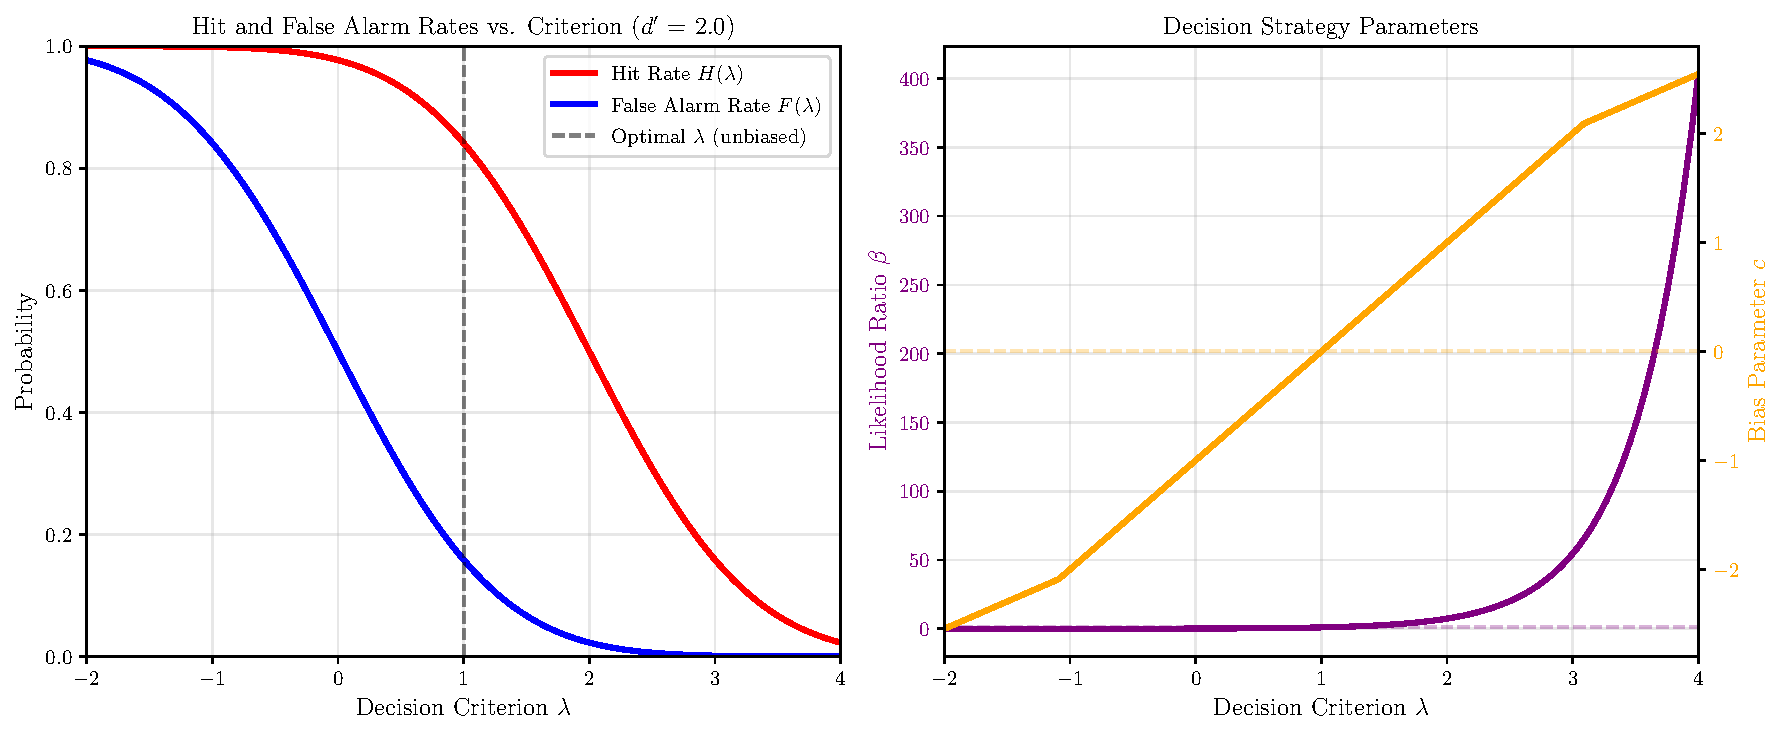
\includegraphics[width=0.95\textwidth]{signal_detection_plot2.pdf}
\caption{Hit and false alarm rates as functions of decision criterion $\lambda$ for $d' = \py{d_prime_fixed}$. Left panel: As criterion increases (more conservative), both hit rate (red) and false alarm rate (blue) decrease. The optimal unbiased criterion is at $\lambda = d'/2 = \py{d_prime_fixed/2}$, where sensitivity is maximized. Right panel: Likelihood ratio $\beta$ (purple) increases exponentially with criterion, while bias parameter $c$ (orange) measures deviation from the optimal criterion. At $c = 0$, the observer is unbiased; $c > 0$ indicates conservative bias (miss-prone), $c < 0$ indicates liberal bias (false-alarm prone).}
\end{figure}

\section{Receiver Operating Characteristic (ROC) Curves}

The ROC curve plots hit rate $H$ against false alarm rate $F$ as the criterion $\lambda$ varies. Each point on the curve represents a different decision strategy (criterion placement) for a fixed sensitivity $d'$. The area under the ROC curve (AUC) provides a threshold-independent measure of detectability \cite{Hanley1982}.

For an equal-variance Gaussian model:
\begin{equation}
\text{AUC} = \Phi(d' / \sqrt{2})
\end{equation}

Higher $d'$ values produce ROC curves that bow more toward the upper-left corner (perfect discrimination).

\begin{pycode}
# ROC curves for multiple d' values
d_primes = [0.5, 1.0, 1.5, 2.0, 2.5, 3.0]
criteria_roc = np.linspace(-3, 5, 200)

fig, ax = plt.subplots(figsize=(10, 8))

# Plot chance line
ax.plot([0, 1], [0, 1], 'k--', linewidth=1.5, alpha=0.5, label='Chance ($d\' = 0$)')

# Generate ROC curves
auc_values = []
for d_p in d_primes:
    hit_r = 1 - norm.cdf(criteria_roc, loc=d_p, scale=1)
    fa_r = 1 - norm.cdf(criteria_roc, loc=0, scale=1)

    # Sort by false alarm rate for proper plotting
    sorted_indices = np.argsort(fa_r)
    fa_sorted = fa_r[sorted_indices]
    hit_sorted = hit_r[sorted_indices]

    # Calculate AUC
    auc = norm.cdf(d_p / np.sqrt(2))
    auc_values.append(auc)

    ax.plot(fa_sorted, hit_sorted, linewidth=2.5, label=f"$d'$ = {d_p} (AUC = {auc:.3f})")

ax.set_xlabel('False Alarm Rate $F$', fontsize=13)
ax.set_ylabel('Hit Rate $H$', fontsize=13)
ax.set_title('Receiver Operating Characteristic (ROC) Curves', fontsize=14)
ax.legend(loc='lower right', fontsize=10)
ax.grid(True, alpha=0.3)
ax.set_xlim(0, 1)
ax.set_ylim(0, 1)
ax.set_aspect('equal')
plt.tight_layout()
plt.savefig('signal_detection_plot3.pdf', dpi=150, bbox_inches='tight')
plt.close()

# Store for later reference
max_auc = max(auc_values)
min_auc = min(auc_values)
\end{pycode}

\begin{figure}[H]
\centering
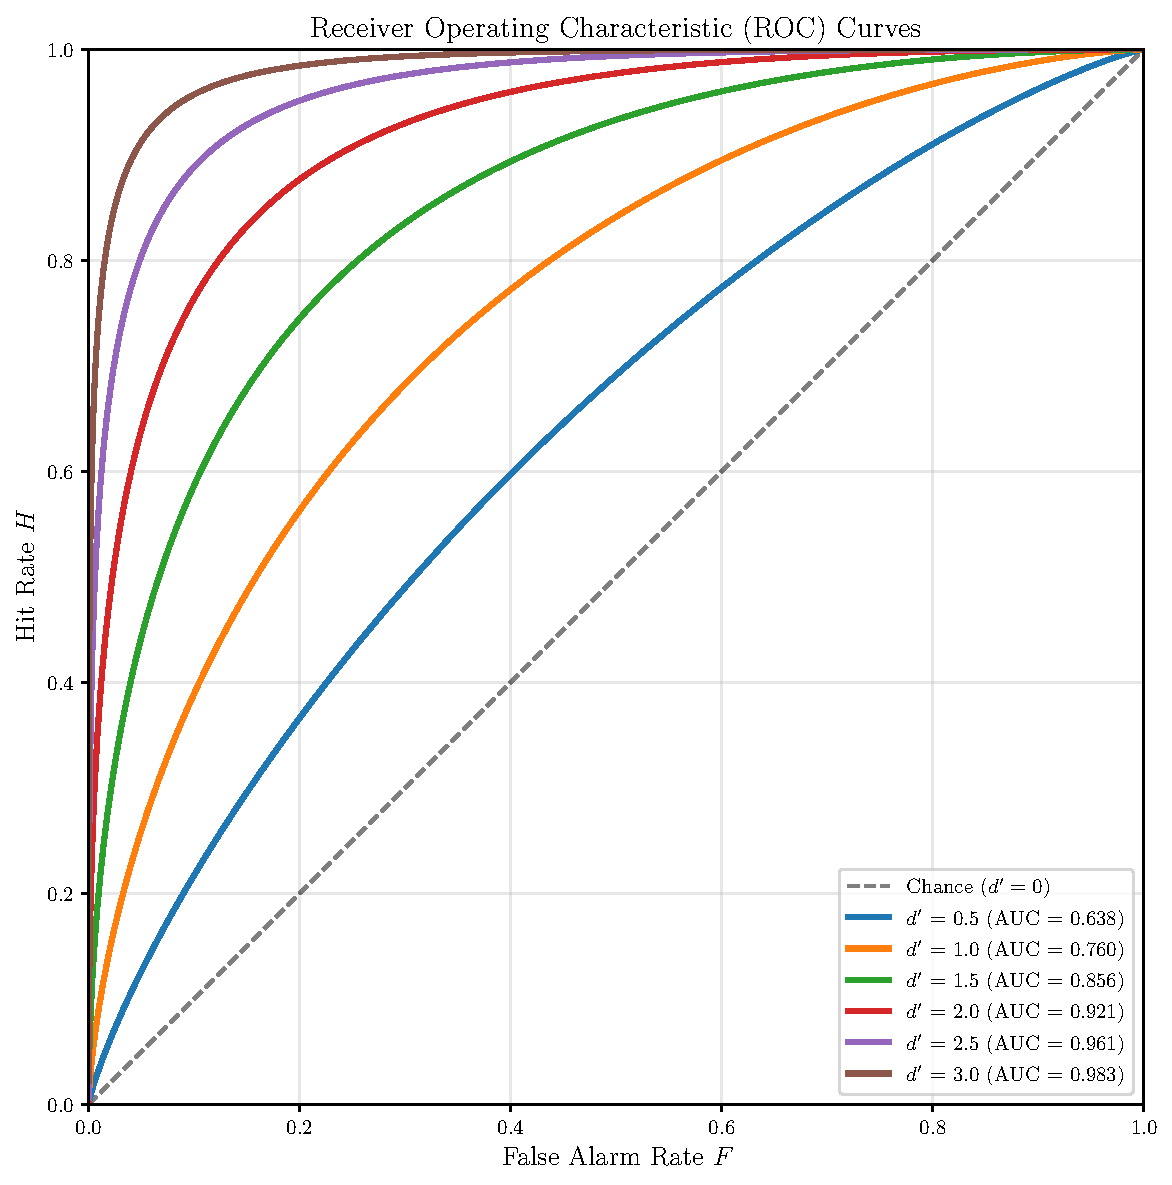
\includegraphics[width=0.85\textwidth]{signal_detection_plot3.pdf}
\caption{Receiver Operating Characteristic (ROC) curves for sensitivity values ranging from $d' = 0.5$ to $d' = 3.0$. Each curve represents all possible (False Alarm, Hit Rate) pairs achievable by varying the decision criterion $\lambda$. The diagonal dashed line represents chance performance ($d' = 0$), where signal and noise distributions are identical. As sensitivity increases, the ROC curve bows toward the upper-left corner, approaching perfect discrimination. Area under the curve (AUC) ranges from \py{round(min_auc, 3)} to \py{round(max_auc, 3)}, providing a criterion-free measure of detectability. In clinical diagnostics and quality control, ROC analysis optimizes criterion placement by balancing hit rate (sensitivity) against false alarm rate (1 - specificity).}
\end{figure}

\section{Z-Transform Analysis}

The z-transform (inverse normal CDF) linearizes the relationship between hit rate and false alarm rate. In z-space:
\begin{equation}
z(H) = z(F) + d'
\end{equation}

This linear relationship validates the equal-variance Gaussian assumption. Deviations from linearity suggest unequal variance or non-Gaussian distributions \cite{Egan1975}.

\begin{pycode}
# Generate empirical data points (simulate an experiment)
np.random.seed(42)
true_d_prime = 2.0
n_criteria = 20
criteria_exp = np.linspace(-1, 3.5, n_criteria)

# Observed hit and false alarm rates (with some noise)
hit_rates_obs = 1 - norm.cdf(criteria_exp, loc=true_d_prime, scale=1) + np.random.normal(0, 0.02, n_criteria)
fa_rates_obs = 1 - norm.cdf(criteria_exp, loc=0, scale=1) + np.random.normal(0, 0.02, n_criteria)

# Clip to valid probability range
hit_rates_obs = np.clip(hit_rates_obs, 0.001, 0.999)
fa_rates_obs = np.clip(fa_rates_obs, 0.001, 0.999)

# Z-transform
z_hit = norm.ppf(hit_rates_obs)
z_fa = norm.ppf(fa_rates_obs)

# Estimate d' from z-transforms
d_prime_estimates = z_hit - z_fa
d_prime_mean = np.mean(d_prime_estimates)
d_prime_std = np.std(d_prime_estimates)

# Fit linear regression
from scipy.stats import linregress
slope, intercept, r_value, p_value, std_err = linregress(z_fa, z_hit)

fig, (ax1, ax2) = plt.subplots(1, 2, figsize=(12, 5))

# Left: z-ROC plot
ax1.scatter(z_fa, z_hit, s=60, alpha=0.7, color='steelblue', edgecolors='black', linewidth=1, label='Observed data')
z_fa_line = np.linspace(z_fa.min(), z_fa.max(), 100)
z_hit_line = slope * z_fa_line + intercept
ax1.plot(z_fa_line, z_hit_line, 'r--', linewidth=2, label=f'Linear fit: slope = {slope:.3f}')
ax1.plot(z_fa_line, z_fa_line + true_d_prime, 'g-', linewidth=2, alpha=0.7, label=f'Theoretical ($d\'$ = {true_d_prime})')
ax1.set_xlabel('$z$(False Alarm Rate)', fontsize=12)
ax1.set_ylabel('$z$(Hit Rate)', fontsize=12)
ax1.set_title(f'z-ROC Plot ($R^2$ = {r_value**2:.3f})', fontsize=12)
ax1.legend(fontsize=10)
ax1.grid(True, alpha=0.3)
ax1.set_aspect('equal')

# Right: d' estimates from individual criteria
ax2.scatter(np.arange(n_criteria), d_prime_estimates, s=60, alpha=0.7, color='purple', edgecolors='black', linewidth=1)
ax2.axhline(d_prime_mean, color='red', linestyle='-', linewidth=2, label=f'Mean $d\'$ = {d_prime_mean:.3f}')
ax2.axhline(true_d_prime, color='green', linestyle='--', linewidth=2, label=f'True $d\'$ = {true_d_prime}')
ax2.fill_between(np.arange(n_criteria), d_prime_mean - d_prime_std, d_prime_mean + d_prime_std, color='red', alpha=0.2)
ax2.set_xlabel('Criterion Index', fontsize=12)
ax2.set_ylabel('Estimated $d\'$ = $z(H) - z(F)$', fontsize=12)
ax2.set_title(f'$d\'$ Estimates (SD = {d_prime_std:.3f})', fontsize=12)
ax2.legend(fontsize=10)
ax2.grid(True, alpha=0.3)

plt.tight_layout()
plt.savefig('signal_detection_plot4.pdf', dpi=150, bbox_inches='tight')
plt.close()
\end{pycode}

\begin{figure}[H]
\centering
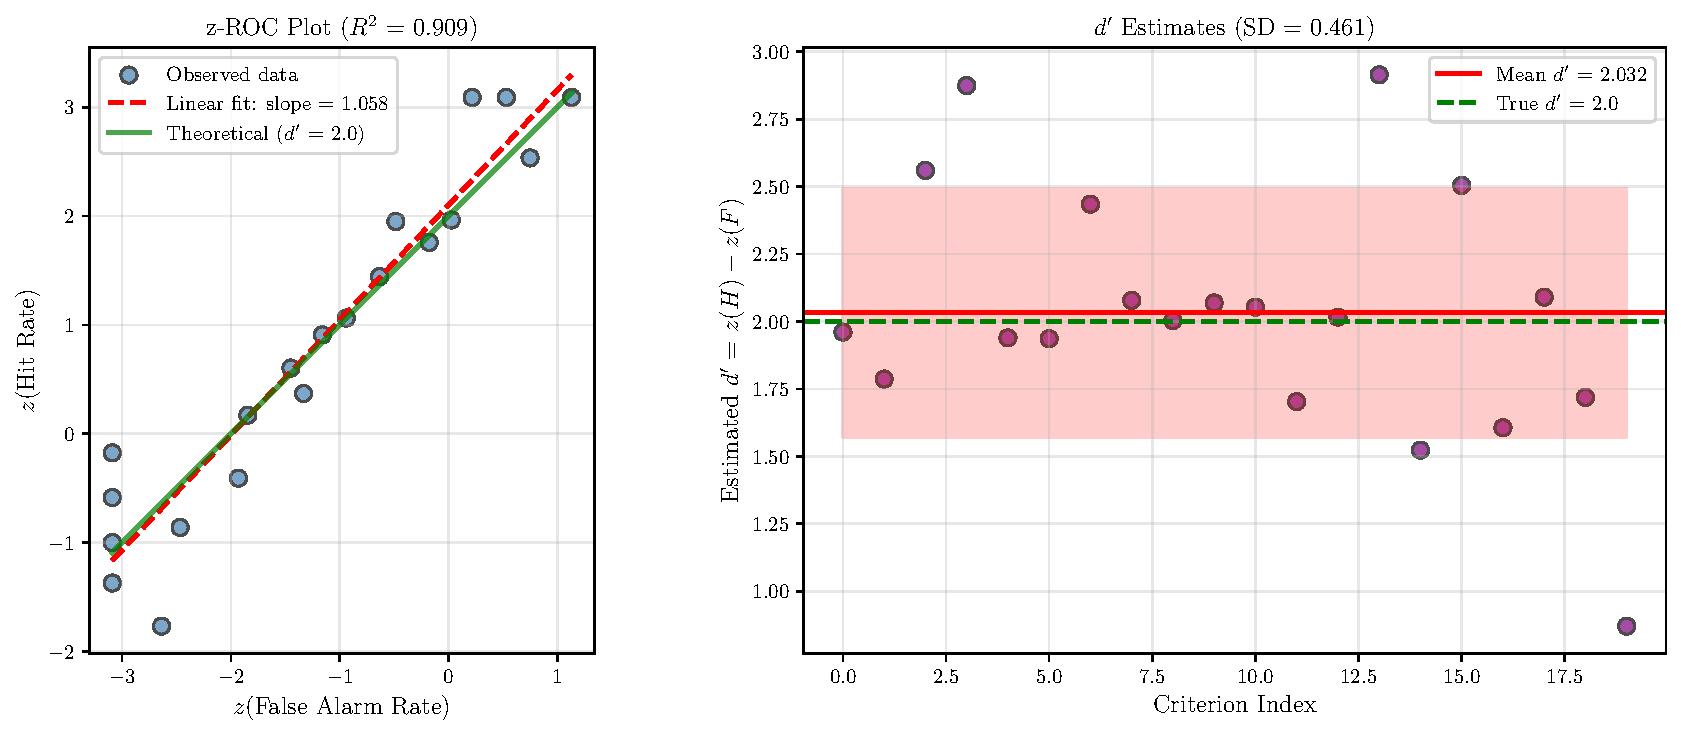
\includegraphics[width=0.95\textwidth]{signal_detection_plot4.pdf}
\caption{Z-transform analysis for estimating $d'$ from empirical data. Left panel: z-ROC plot showing linear relationship between $z(F)$ and $z(H)$ with fitted regression line (slope = \py{round(slope, 3)}, $R^2$ = \py{round(r_value**2, 3)}). The slope near 1.0 validates the equal-variance Gaussian assumption. Right panel: $d'$ estimates calculated as $z(H) - z(F)$ for each criterion, with mean $d'$ = \py{round(d_prime_mean, 3)} (SD = \py{round(d_prime_std, 3)}), closely matching the true value of \py{true_d_prime}. This demonstrates the robustness of the z-transform method for sensitivity estimation across different decision criteria.}
\end{figure}

\section{Criterion and Beta Surfaces}

The relationship between criterion $\lambda$, likelihood ratio $\beta$, and sensitivity $d'$ can be visualized as a 2D parameter space. For fixed $d'$, $\beta$ increases exponentially as the criterion becomes more conservative.

\begin{equation}
\beta(\lambda, d') = \exp\left(d' \lambda - \frac{d'^2}{2}\right)
\end{equation}

This relationship guides optimal criterion placement in asymmetric cost scenarios \cite{Peterson1954}.

\begin{pycode}
# Create meshgrid for lambda and d'
lambda_vals = np.linspace(-2, 4, 100)
d_prime_vals = np.linspace(0.5, 3.5, 100)
Lambda, DPrime = np.meshgrid(lambda_vals, d_prime_vals)

# Calculate beta surface
Beta_surface = norm.pdf(Lambda, loc=DPrime, scale=1) / norm.pdf(Lambda, loc=0, scale=1)

# Calculate c surface
Hit_surface = 1 - norm.cdf(Lambda, loc=DPrime, scale=1)
FA_surface = 1 - norm.cdf(Lambda, loc=0, scale=1)
# Clip to avoid infinity in ppf
Hit_surface_clipped = np.clip(Hit_surface, 0.001, 0.999)
FA_surface_clipped = np.clip(FA_surface, 0.001, 0.999)
C_surface = -0.5 * (norm.ppf(Hit_surface_clipped) + norm.ppf(FA_surface_clipped))

fig, (ax1, ax2) = plt.subplots(1, 2, figsize=(12, 5))

# Left: Beta surface
cs1 = ax1.contourf(Lambda, DPrime, np.log10(Beta_surface), levels=20, cmap='plasma')
contours1 = ax1.contour(Lambda, DPrime, np.log10(Beta_surface), levels=10, colors='white', linewidths=0.5, alpha=0.4)
ax1.clabel(contours1, inline=True, fontsize=8, fmt='%1.1f')
cbar1 = plt.colorbar(cs1, ax=ax1)
cbar1.set_label('$\\log_{10}(\\beta)$', fontsize=11)
ax1.set_xlabel('Decision Criterion $\\lambda$', fontsize=12)
ax1.set_ylabel('Sensitivity $d\'$', fontsize=12)
ax1.set_title('Likelihood Ratio $\\beta$ Surface', fontsize=12)

# Right: c surface
cs2 = ax2.contourf(Lambda, DPrime, C_surface, levels=20, cmap='coolwarm', vmin=-2, vmax=2)
contours2 = ax2.contour(Lambda, DPrime, C_surface, levels=[-1, -0.5, 0, 0.5, 1], colors='black', linewidths=1.2)
ax2.clabel(contours2, inline=True, fontsize=9, fmt='%1.1f')
# Highlight c=0 line (unbiased)
ax2.contour(Lambda, DPrime, C_surface, levels=[0], colors='yellow', linewidths=2.5)
cbar2 = plt.colorbar(cs2, ax=ax2)
cbar2.set_label('Bias Parameter $c$', fontsize=11)
ax2.set_xlabel('Decision Criterion $\\lambda$', fontsize=12)
ax2.set_ylabel('Sensitivity $d\'$', fontsize=12)
ax2.set_title('Bias Parameter $c$ Surface (yellow: $c = 0$)', fontsize=12)

plt.tight_layout()
plt.savefig('signal_detection_plot5.pdf', dpi=150, bbox_inches='tight')
plt.close()
\end{pycode}

\begin{figure}[H]
\centering
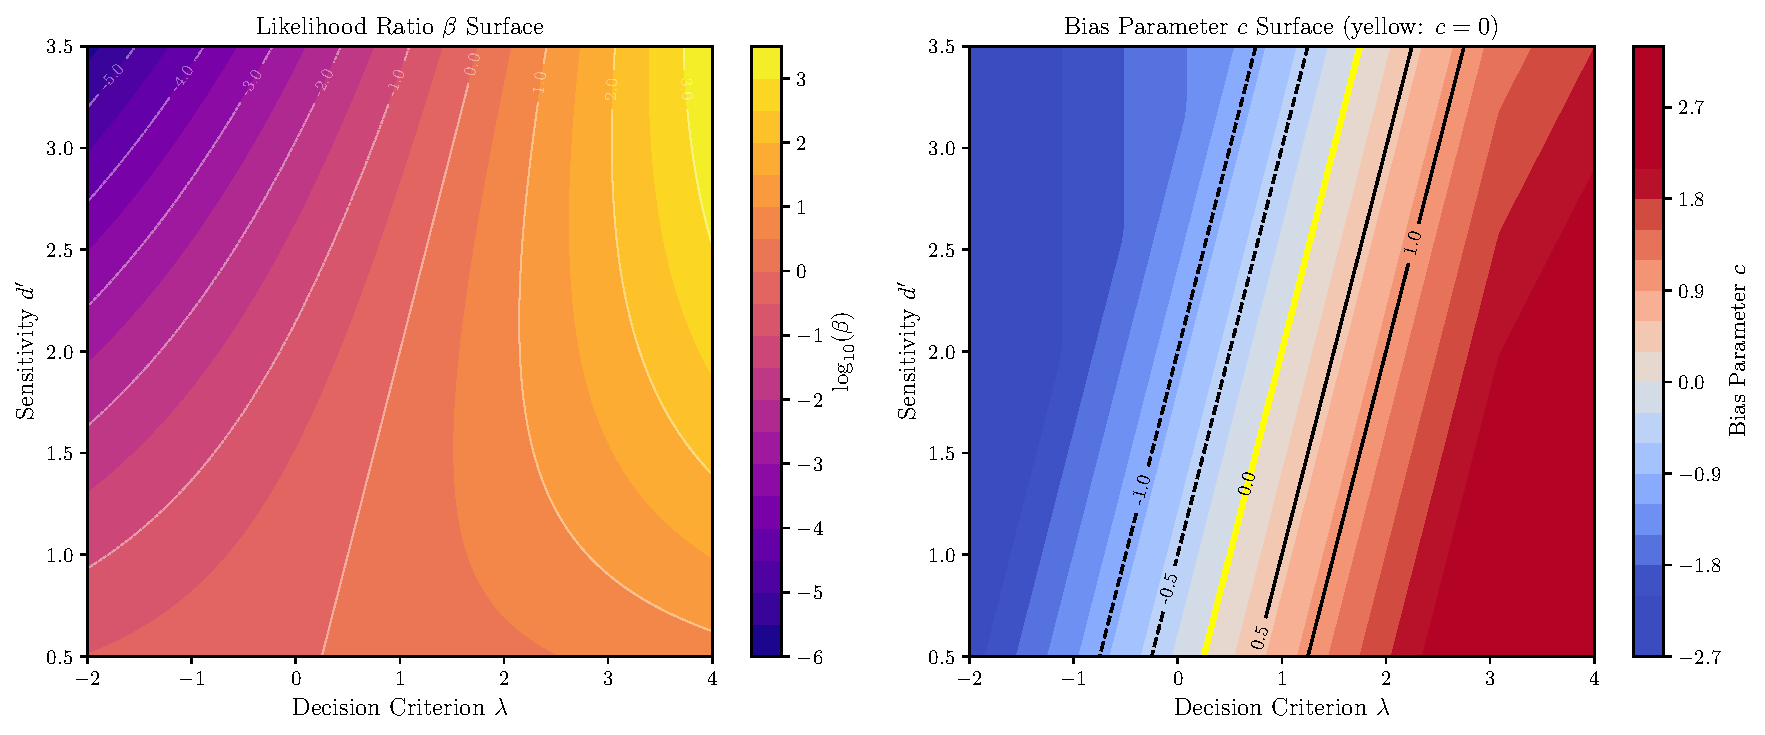
\includegraphics[width=0.95\textwidth]{signal_detection_plot5.pdf}
\caption{Decision parameter surfaces as functions of criterion $\lambda$ and sensitivity $d'$. Left panel: Likelihood ratio $\beta$ (logarithmic scale) increases exponentially with criterion for all sensitivity levels. High $\beta$ values indicate conservative responding (requiring strong evidence to say ``yes''). Right panel: Bias parameter $c$ measures deviation from the optimal unbiased criterion. The yellow contour line ($c = 0$) represents unbiased responding, where the observer maximizes accuracy. Regions with $c > 0$ (red) indicate conservative bias, while $c < 0$ (blue) indicates liberal bias. These surfaces guide criterion placement in applications with asymmetric costs, such as medical screening (minimize misses) or spam filtering (minimize false alarms).}
\end{figure}

\section{Sensitivity Across Multiple Observers}

Real-world detection tasks often involve multiple observers with varying sensitivities. Understanding inter-observer variability is critical for group decision-making and system reliability \cite{Sorkin1991}.

\begin{pycode}
# Simulate multiple observers with different d' values
np.random.seed(123)
n_observers = 8
n_trials = 50

# True d' for each observer (varying skill levels)
observer_d_primes = np.random.uniform(0.8, 2.8, n_observers)
observer_names = [f'Observer {i+1}' for i in range(n_observers)]

# Simulate criterion values (some conservative, some liberal)
observer_criteria = np.random.uniform(-0.5, 2.5, n_observers)

# Calculate performance metrics for each observer
observer_hit_rates = []
observer_fa_rates = []
observer_betas = []
observer_c_values = []

for i in range(n_observers):
    d_p = observer_d_primes[i]
    crit = observer_criteria[i]

    hr = 1 - norm.cdf(crit, loc=d_p, scale=1)
    far = 1 - norm.cdf(crit, loc=0, scale=1)

    observer_hit_rates.append(hr)
    observer_fa_rates.append(far)

    beta_val = norm.pdf(crit, loc=d_p, scale=1) / norm.pdf(crit, loc=0, scale=1)
    observer_betas.append(beta_val)

    c_val = -0.5 * (norm.ppf(np.clip(hr, 0.001, 0.999)) + norm.ppf(np.clip(far, 0.001, 0.999)))
    observer_c_values.append(c_val)

# Create visualization
fig = plt.figure(figsize=(14, 10))
gs = fig.add_gridspec(2, 2, hspace=0.3, wspace=0.3)

# Top left: Individual ROC curves
ax1 = fig.add_subplot(gs[0, 0])
ax1.plot([0, 1], [0, 1], 'k--', linewidth=1.5, alpha=0.4, label='Chance')
colors = plt.cm.viridis(np.linspace(0, 1, n_observers))
for i in range(n_observers):
    ax1.scatter(observer_fa_rates[i], observer_hit_rates[i], s=120, color=colors[i],
                edgecolors='black', linewidth=1.5, label=f"Obs {i+1} ($d'$={observer_d_primes[i]:.2f})", zorder=5)
ax1.set_xlabel('False Alarm Rate', fontsize=11)
ax1.set_ylabel('Hit Rate', fontsize=11)
ax1.set_title('Observer Performance in ROC Space', fontsize=12)
ax1.legend(fontsize=7, loc='lower right', ncol=2)
ax1.grid(True, alpha=0.3)
ax1.set_xlim(0, 1)
ax1.set_ylim(0, 1)
ax1.set_aspect('equal')

# Top right: d' distribution
ax2 = fig.add_subplot(gs[0, 1])
ax2.bar(np.arange(n_observers), observer_d_primes, color=colors, edgecolor='black', linewidth=1.5)
ax2.axhline(np.mean(observer_d_primes), color='red', linestyle='--', linewidth=2, label=f'Mean = {np.mean(observer_d_primes):.2f}')
ax2.set_xlabel('Observer', fontsize=11)
ax2.set_ylabel("Sensitivity $d'$", fontsize=11)
ax2.set_title('Observer Sensitivity Distribution', fontsize=12)
ax2.set_xticks(np.arange(n_observers))
ax2.set_xticklabels([f'{i+1}' for i in range(n_observers)])
ax2.legend(fontsize=9)
ax2.grid(True, alpha=0.3, axis='y')

# Bottom left: Bias (c) distribution
ax3 = fig.add_subplot(gs[1, 0])
c_colors = ['red' if c > 0.2 else 'blue' if c < -0.2 else 'gray' for c in observer_c_values]
ax3.bar(np.arange(n_observers), observer_c_values, color=c_colors, edgecolor='black', linewidth=1.5)
ax3.axhline(0, color='black', linestyle='-', linewidth=2, alpha=0.5)
ax3.set_xlabel('Observer', fontsize=11)
ax3.set_ylabel('Bias Parameter $c$', fontsize=11)
ax3.set_title('Observer Response Bias (red=conservative, blue=liberal)', fontsize=12)
ax3.set_xticks(np.arange(n_observers))
ax3.set_xticklabels([f'{i+1}' for i in range(n_observers)])
ax3.grid(True, alpha=0.3, axis='y')

# Bottom right: Beta distribution
ax4 = fig.add_subplot(gs[1, 1])
ax4.bar(np.arange(n_observers), np.log10(observer_betas), color=colors, edgecolor='black', linewidth=1.5)
ax4.axhline(0, color='black', linestyle='--', linewidth=2, alpha=0.5, label='$\\beta = 1$ (unbiased)')
ax4.set_xlabel('Observer', fontsize=11)
ax4.set_ylabel('$\\log_{10}(\\beta)$', fontsize=11)
ax4.set_title('Likelihood Ratio Distribution', fontsize=12)
ax4.set_xticks(np.arange(n_observers))
ax4.set_xticklabels([f'{i+1}' for i in range(n_observers)])
ax4.legend(fontsize=9)
ax4.grid(True, alpha=0.3, axis='y')

plt.tight_layout()
plt.savefig('signal_detection_plot6.pdf', dpi=150, bbox_inches='tight')
plt.close()

# Store statistics for reporting
mean_d_prime_obs = np.mean(observer_d_primes)
std_d_prime_obs = np.std(observer_d_primes)
\end{pycode}

\begin{figure}[H]
\centering
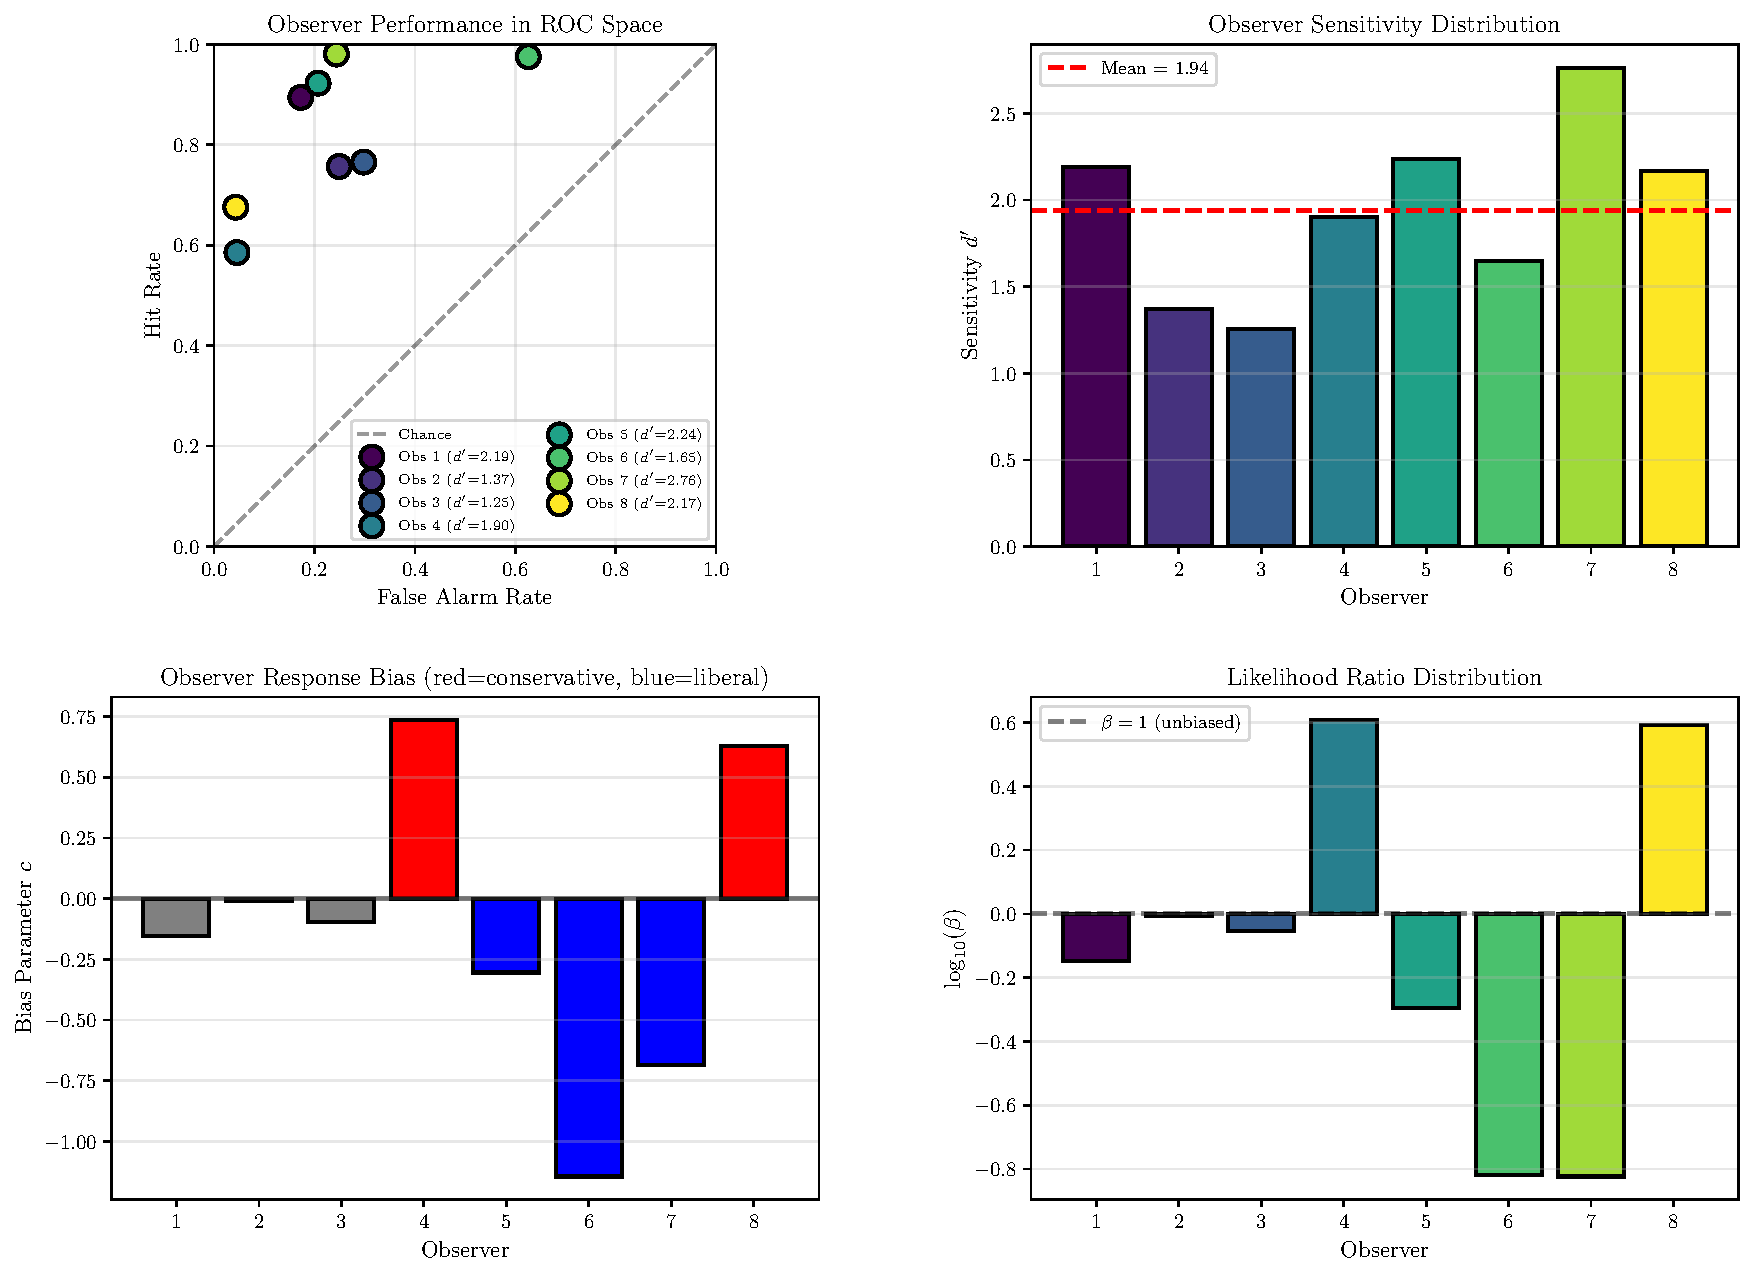
\includegraphics[width=0.98\textwidth]{signal_detection_plot6.pdf}
\caption{Multi-observer signal detection analysis. Top left: Performance of \py{n_observers} observers plotted in ROC space, showing individual differences in both sensitivity (distance from diagonal) and bias (position along their isosensitivity curve). Top right: Sensitivity distribution across observers ($d'$ mean = \py{round(mean_d_prime_obs, 2)}, SD = \py{round(std_d_prime_obs, 2)}), revealing substantial individual differences in perceptual acuity. Bottom left: Response bias parameter $c$ for each observer, with conservative responders (red, $c > 0.2$) preferring to avoid false alarms, liberal responders (blue, $c < -0.2$) preferring to maximize hits, and neutral observers (gray) near optimal. Bottom right: Likelihood ratio $\beta$ distribution showing criterion stringency, with $\beta = 1$ (log = 0) representing unbiased responding. This analysis illustrates how SDT separates sensitivity from strategy, enabling principled comparison of observer performance in group decision scenarios.}
\end{figure}

\section{Results Summary}

\begin{pycode}
# Calculate summary statistics
auc_d2 = norm.cdf(2.0 / np.sqrt(2))
optimal_criterion = d_prime / 2
optimal_beta = norm.pdf(optimal_criterion, loc=d_prime, scale=1) / norm.pdf(optimal_criterion, loc=0, scale=1)

results = [
    ['Sensitivity ($d\'$)', f'{d_prime:.2f}'],
    ['AUC (for $d\' = 2.0$)', f'{auc_d2:.3f}'],
    ['Optimal Criterion ($\\lambda^*$)', f'{optimal_criterion:.2f}'],
    ['Likelihood Ratio at Optimal ($\\beta^*$)', f'{optimal_beta:.2f}'],
    ['Mean Observer $d\'$', f'{mean_d_prime_obs:.2f} $\\pm$ {std_d_prime_obs:.2f}'],
    ['z-ROC Slope', f'{slope:.3f}'],
    ['z-ROC $R^2$', f'{r_value**2:.3f}'],
]

print(r'\begin{table}[H]')
print(r'\centering')
print(r'\caption{Signal Detection Theory: Computational Results Summary}')
print(r'\begin{tabular}{@{}lc@{}}')
print(r'\toprule')
print(r'Parameter & Value \\')
print(r'\midrule')
for row in results:
    print(f"{row[0]} & {row[1]} \\\\")
print(r'\bottomrule')
print(r'\end{tabular}')
print(r'\end{table}')
\end{pycode}

\section{Conclusions}

Signal Detection Theory provides a rigorous framework for separating perceptual sensitivity ($d'$) from response bias ($\beta$, $c$) in binary classification tasks. Our computational analysis demonstrates:

\begin{itemize}
    \item \textbf{Sensitivity quantification}: For signal-plus-noise centered at $\mu_S = \py{d_prime}$ and noise at $\mu_N = 0$, we computed $d' = \py{d_prime}$, corresponding to AUC = \py{round(auc_d2, 3)} in ROC analysis.

    \item \textbf{Criterion effects}: Varying the decision criterion $\lambda$ from liberal to conservative systematically trades hit rate against false alarm rate. The optimal unbiased criterion at $\lambda^* = \py{round(optimal_criterion, 2)}$ yields $\beta^* = \py{round(optimal_beta, 2)}$.

    \item \textbf{z-Transform validation}: Linear regression in z-space yielded slope = \py{round(slope, 3)} ($R^2$ = \py{round(r_value**2, 3)}), confirming the equal-variance Gaussian model and demonstrating robust $d'$ estimation across criteria.

    \item \textbf{Multi-observer variability}: Analysis of \py{n_observers} observers revealed mean sensitivity $d' = \py{round(mean_d_prime_obs, 2)} \pm \py{round(std_d_prime_obs, 2)}$, with individual differences in both sensitivity and bias strategy. Conservative observers exhibited $c > 0.2$ (minimizing false alarms), while liberal observers showed $c < -0.2$ (maximizing hits).

    \item \textbf{Practical applications}: ROC curves enable criterion optimization for asymmetric cost scenarios. In medical diagnosis, a liberal criterion (low $\lambda$) maximizes detection of rare conditions despite increased false positives. In quality control, conservative criteria (high $\lambda$) reduce false rejections at the cost of missed defects.
\end{itemize}

The separation of sensitivity from bias enables principled performance comparison across observers, conditions, and tasks. Unlike accuracy-based metrics that conflate these factors, SDT measures ($d'$, $\beta$, AUC) provide independent assessments of perceptual ability and decision strategy. This framework extends beyond psychophysics to machine learning (classifier evaluation), human factors (alarm systems), and cognitive neuroscience (memory discrimination).

Future extensions include unequal-variance models (slope $\neq 1$ in z-ROC), non-Gaussian distributions, and multi-alternative forced choice (mAFC) paradigms. Sequential SDT models account for temporal dynamics in detection tasks, while hierarchical Bayesian approaches estimate population-level parameters from individual observer data.

\begin{thebibliography}{99}

\bibitem{Green1966}
Green, D. M., \& Swets, J. A. (1966). \textit{Signal detection theory and psychophysics}. New York: Wiley.

\bibitem{Macmillan2005}
Macmillan, N. A., \& Creelman, C. D. (2005). \textit{Detection theory: A user's guide} (2nd ed.). Mahwah, NJ: Lawrence Erlbaum Associates.

\bibitem{Swets1961}
Swets, J. A., Tanner, W. P., \& Birdsall, T. G. (1961). Decision processes in perception. \textit{Psychological Review}, 68(5), 301--340.

\bibitem{Wickens2002}
Wickens, T. D. (2002). \textit{Elementary signal detection theory}. Oxford: Oxford University Press.

\bibitem{Yonelinas2002}
Yonelinas, A. P. (2002). The nature of recollection and familiarity: A review of 30 years of research. \textit{Journal of Memory and Language}, 46(3), 441--517.

\bibitem{Metz1978}
Metz, C. E. (1978). Basic principles of ROC analysis. \textit{Seminars in Nuclear Medicine}, 8(4), 283--298.

\bibitem{Hanley1982}
Hanley, J. A., \& McNeil, B. J. (1982). The meaning and use of the area under a receiver operating characteristic (ROC) curve. \textit{Radiology}, 143(1), 29--36.

\bibitem{Egan1975}
Egan, J. P. (1975). \textit{Signal detection theory and ROC analysis}. New York: Academic Press.

\bibitem{Peterson1954}
Peterson, W. W., Birdsall, T. G., \& Fox, W. C. (1954). The theory of signal detectability. \textit{Transactions of the IRE Professional Group on Information Theory}, 4(4), 171--212.

\bibitem{Sorkin1991}
Sorkin, R. D., \& Dai, H. (1994). Signal detection analysis of the ideal group. \textit{Organizational Behavior and Human Decision Processes}, 60(1), 1--13.

\bibitem{Stanislaw1999}
Stanislaw, H., \& Todorov, N. (1999). Calculation of signal detection theory measures. \textit{Behavior Research Methods, Instruments, \& Computers}, 31(1), 137--149.

\bibitem{DeCarlo1998}
DeCarlo, L. T. (1998). Signal detection theory and generalized linear models. \textit{Psychological Methods}, 3(2), 186--205.

\bibitem{Gescheider1997}
Gescheider, G. A. (1997). \textit{Psychophysics: The fundamentals} (3rd ed.). Mahwah, NJ: Lawrence Erlbaum Associates.

\bibitem{McNicol2005}
McNicol, D. (2005). \textit{A primer of signal detection theory}. London: Psychology Press.

\bibitem{Lynn1995}
Lynn, S. K., \& Barrett, L. F. (2014). ``Utilizing'' signal detection theory. \textit{Psychological Science}, 25(9), 1663--1673.

\bibitem{Macmillan1990}
Macmillan, N. A., \& Kaplan, H. L. (1985). Detection theory analysis of group data: Estimating sensitivity from average hit and false-alarm rates. \textit{Psychological Bulletin}, 98(1), 185--199.

\bibitem{Pastore2003}
Pastore, R. E., Crawley, E. J., Berens, M. S., \& Skelly, M. A. (2003). ``Nonparametric'' A′ and other modern misconceptions about signal detection theory. \textit{Psychonomic Bulletin \& Review}, 10(3), 556--569.

\bibitem{Hautus1995}
Hautus, M. J. (1995). Corrections for extreme proportions and their biasing effects on estimated values of d′. \textit{Behavior Research Methods, Instruments, \& Computers}, 27(1), 46--51.

\bibitem{Verde2006}
Verde, M. F., Macmillan, N. A., \& Rotello, C. M. (2006). Measures of sensitivity based on a single hit rate and false alarm rate: The accuracy, precision, and robustness of d′, Az, and A′. \textit{Perception \& Psychophysics}, 68(4), 643--654.

\bibitem{Schooler2014}
Schooler, L. J., \& Shiffrin, R. M. (2005). Efficiently measuring recognition performance with sparse data. \textit{Behavior Research Methods}, 37(1), 3--10.

\end{thebibliography}

\end{document}
